\section{Introduction}

This sprint focuses on the scanning pipeline and on the vulnerability processing features of the HexStrike platform. The goal of this iteration is to implement reliable scan orchestration, normalize heterogeneous tool outputs into a unified schema, match findings against the vulnerability catalog, and persist results for later analysis and reporting.

In practice, this sprint covers scan submission, queueing and scheduling, worker orchestration, normalization, vulnerability matching, result persistence, and the user interfaces to submit and view scans.

\subsection{Sprint Purpose}

The purpose of this sprint is to deliver a robust scan processing pipeline that reliably executes scanners, normalizes their outputs, matches findings to known vulnerabilities, and stores results for retrieval and analysis. Success is measured by correct job processing, normalized result coverage for representative tool outputs, accurate matching to the catalog, and end-to-end retrieval from the UI.

\section{Sprint Backlog}

The backlog for this sprint contains the following user stories:

\begin{table}[H]
    \centering
    \renewcommand{\arraystretch}{1.2}
    \begin{tabularx}{\textwidth}{|X|}
        \hline
        As a user, I can submit a scan target (URL) and receive a job identifier. \\\hline
        As a user, I can schedule or queue scans for later execution. \\\hline
        As the system, I can run scanner tools and collect raw outputs. \\\hline
        As the system, I can normalize raw outputs into a unified \texttt{ScanResult} schema. \\\hline
        As the system, I can match normalized findings to the vulnerability catalog and assign severities. \\\hline
        As a user, I can view, filter, and export scan history and results. \\\hline
        As an operator, I can monitor queue status and worker health. \\\hline
    \end{tabularx}
    \caption{Sprint Backlog}
\end{table}

\section{Requirements Analysis}

\subsection{Use Case Diagram}

The primary actors are the authenticated user (or guest if allowed), the API, and the scan worker. The use case diagram illustrates submission, processing, normalization, matching and viewing flows.

\begin{figure}[H]
    \centering
    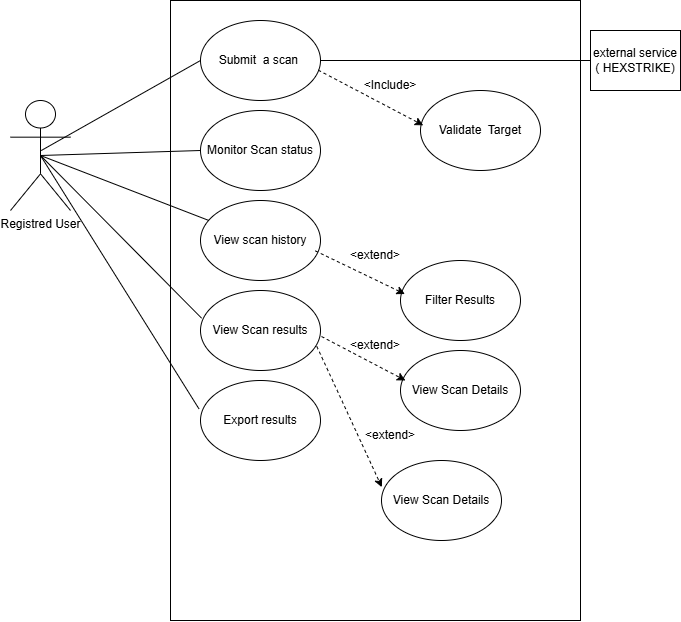
\includegraphics[width=0.9\textwidth]{uploads/diagrams/sprint2 usecas.drawio.png}
    \caption{Use case diagram for scanning and vulnerability processing}
    \label{fig:sprint4-usecase}
\end{figure}

\subsection{Use Case Description}

The main use cases of this sprint are summarized in the following tables.

\begin{table}[H]
    \centering
    \renewcommand{\arraystretch}{1.2}
    \begin{tabular}{|p{3cm}|p{11cm}|}
        \hline
        \textbf{Use case} & Submit Scan \\ \hline
        \textbf{Actor} & Authenticated user (or Guest if permitted) \\ \hline
        \textbf{Description} & The user provides a target (URL) and optional parameters; the backend validates input, creates a \texttt{Scan} job, enqueues it and returns a job identifier. \\ \hline
        \textbf{Pre-condition} & The user is authorized to submit scans and the queue service is available. \\ \hline
        \textbf{Post-condition} & A \texttt{Scan} job is stored and queued for processing; the user receives the job id. \\ \hline
    \end{tabular}
    \caption{Use case description: Submit Scan}
    \label{tab:submit-scan}
\end{table}





\begin{table}[H]
    \centering
    \renewcommand{\arraystretch}{1.2}
    \begin{tabular}{|p{3cm}|p{11cm}|}
        \hline
        \textbf{Use case} & View Scan History \\ \hline
        \textbf{Actor} & Authenticated user \\ \hline
        \textbf{Description} & The user requests a list of past scans, applies filters, and inspects a scan's details and matched vulnerabilities. \\ \hline
        \textbf{Pre-condition} & Scan results have been persisted and the user is authorized to view them. \\ \hline
        \textbf{Post-condition} & The requested data is displayed; the user may export or navigate to details. \\ \hline
    \end{tabular}
    \caption{Use case description: View Scan History}
    \label{tab:view-history}
\end{table}

\begin{table}[H]
    \centering
    \renewcommand{\arraystretch}{1.2}
    \begin{tabular}{|p{3cm}|p{11cm}|}
        \hline
        \textbf{Use case} & View / Browse scan results \\ \hline
        \textbf{Actor} & Authenticated user \\ \hline
        \textbf{Description} & The user selects a completed scan to view its results. The system displays scan metadata including target URL, scan date, scan configuration, and execution summary. It also shows a detailed list of discovered vulnerabilities with severity, affected paths, CVE or reference identifiers, and brief remediation notes. \\ \hline
        \textbf{Pre-condition} & One or more completed scans exist and the user has permission to view them. \\ \hline
        \textbf{Post-condition} & Scan metadata and vulnerabilities are presented to the user; the user may drill down into individual findings or export the data. \\ \hline
    \end{tabular}
    \caption{Use case description: View / Browse scan results}
    \label{tab:view-results-usecase}
\end{table}

\begin{table}[H]
    \centering
    \renewcommand{\arraystretch}{1.2}
    \begin{tabular}{|p{3cm}|p{11cm}|}
        \hline
        \textbf{Use case} & Scan report exporting \\ \hline
        \textbf{Actor} & Authenticated user \\ \hline
        \textbf{Description} & The user requests an export of a completed scan report. The system generates an export file (PDF, CSV or JSON) that includes scan metadata, a summary of findings, detailed vulnerability entries, and optional attachments (screenshots, raw tool outputs). The user can download the file or receive it via email. \\ \hline
        \textbf{Pre-condition} & A completed scan exists and the user has permission to export reports. \\ \hline
        \textbf{Post-condition} & An export file is generated and made available to the user; export operations are logged for audit. \\ \hline
    \end{tabular}
    \caption{Use case description: Scan report exporting}
    \label{tab:scan-export-usecase}
\end{table}

\section{Design}

\subsection{Class Diagram}

The principal components include the API, the queue, worker processes, the normalizer and matcher services, and the persistence layer. The class diagram will show the data models and service classes.

\begin{figure}[H]
    \centering
    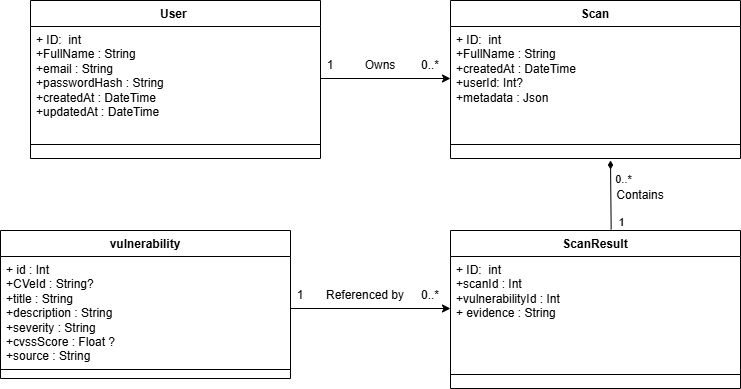
\includegraphics[width=0.98\textwidth]{uploads/diagrams/sprint 2 classe diagram.drawio.png}
    \caption{Class diagram for Sprint 2}
    \label{fig:sprint4-class-diagram}
\end{figure}

\subsection{Scan Workflow}

The scan workflow describes the end-to-end processing of a submitted target: submission, queueing, worker execution of tools, normalization, matching, and persistence. The diagram below summarizes the sequence and components involved.

\begin{figure}[H]
    \centering
    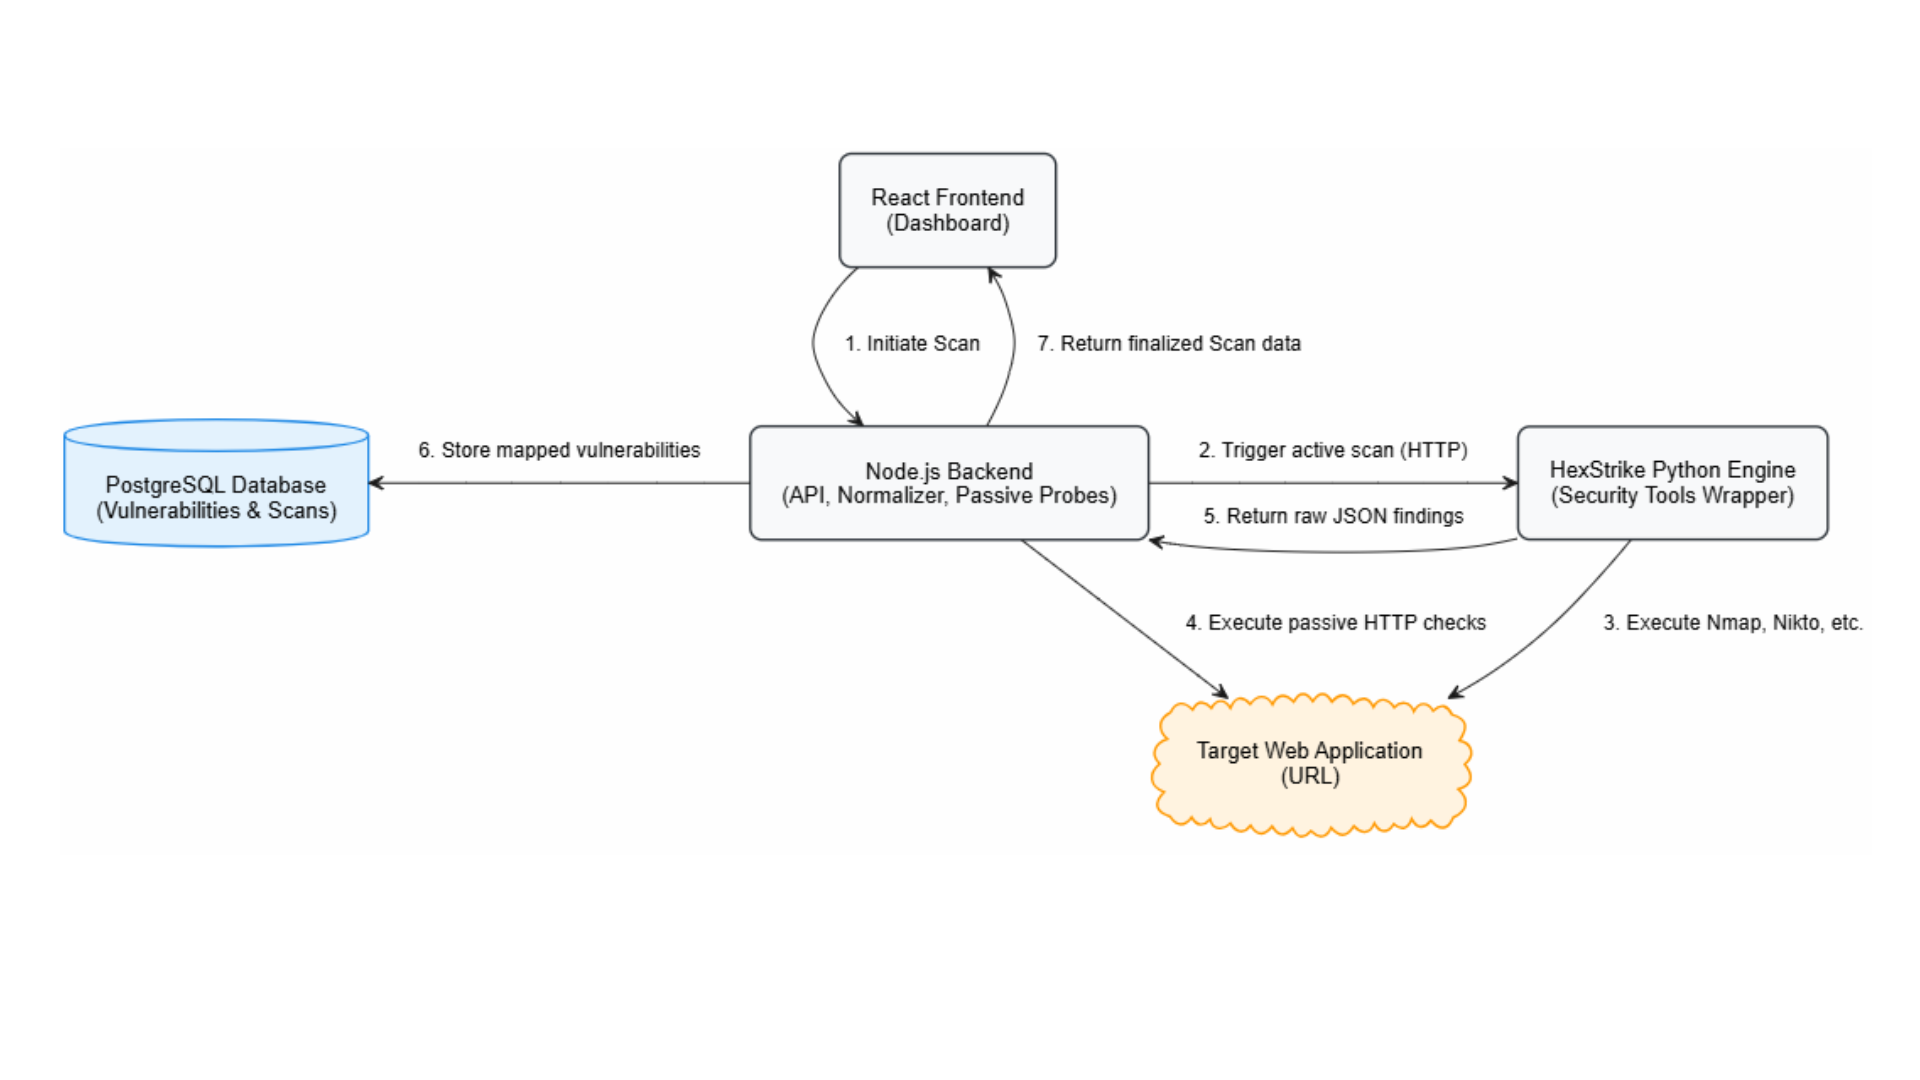
\includegraphics[width=0.9\textwidth]{uploads/diagrams/scan pipline.png}
    \caption{Scan workflow overview}
    \label{fig:scan-workflow}
\end{figure}

\subsection{Sequence Diagram}

Key sequences include submission-to-persistence and normalization-to-matching. A sequence diagram will illustrate the interactions between client, API, queue, worker, normalizer, matcher and DB.

\begin{figure}[H]
    \centering
    
\includegraphics[width=0.98\textwidth]{uploads/diagrams/sprint2 sequence.drawio (3).png}
    \caption{Sequence diagram for scan processing}
    \label{fig:sprint4-sequence-diagram}
\end{figure}

\section{Implementation}

In this sprint, we present the interfaces developed for Sprint 2. The implementation includes the scanner submission interface,  scan history with filtering options, and detailed scan results view. The following figures illustrate the application interfaces:

\begin{figure}[H]
    \centering
    \fbox{\parbox{0.85\textwidth}{\centering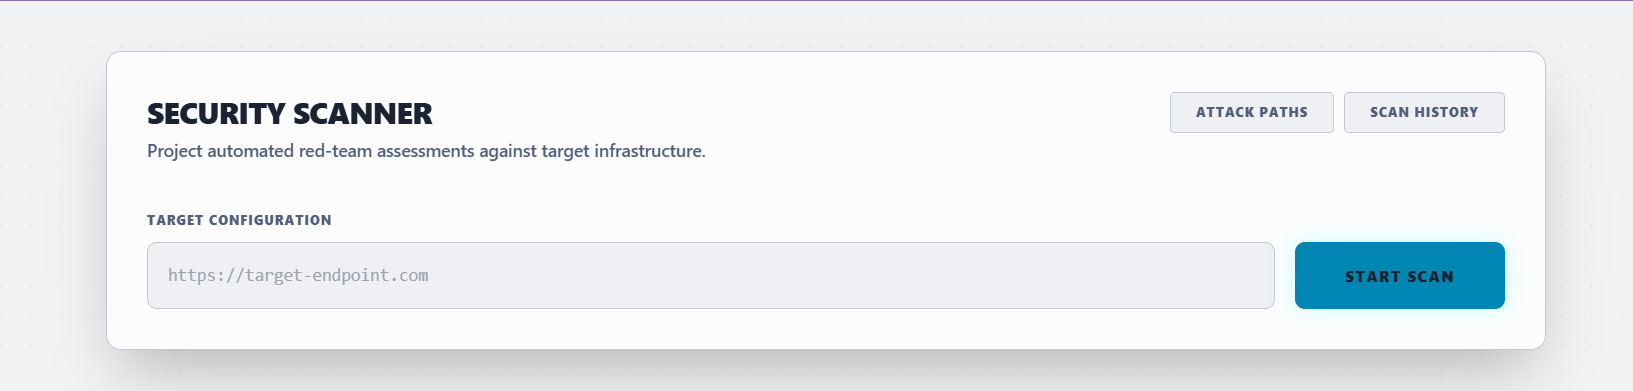
\includegraphics[width=0.85\textwidth]{uploads/images/scan.png}}}% 
    \caption{Scanner submission page}
    \label{fig:scanner4-page}
\end{figure}

\begin{figure}[H]
    \centering
    \fbox{\parbox{0.85\textwidth}{\centering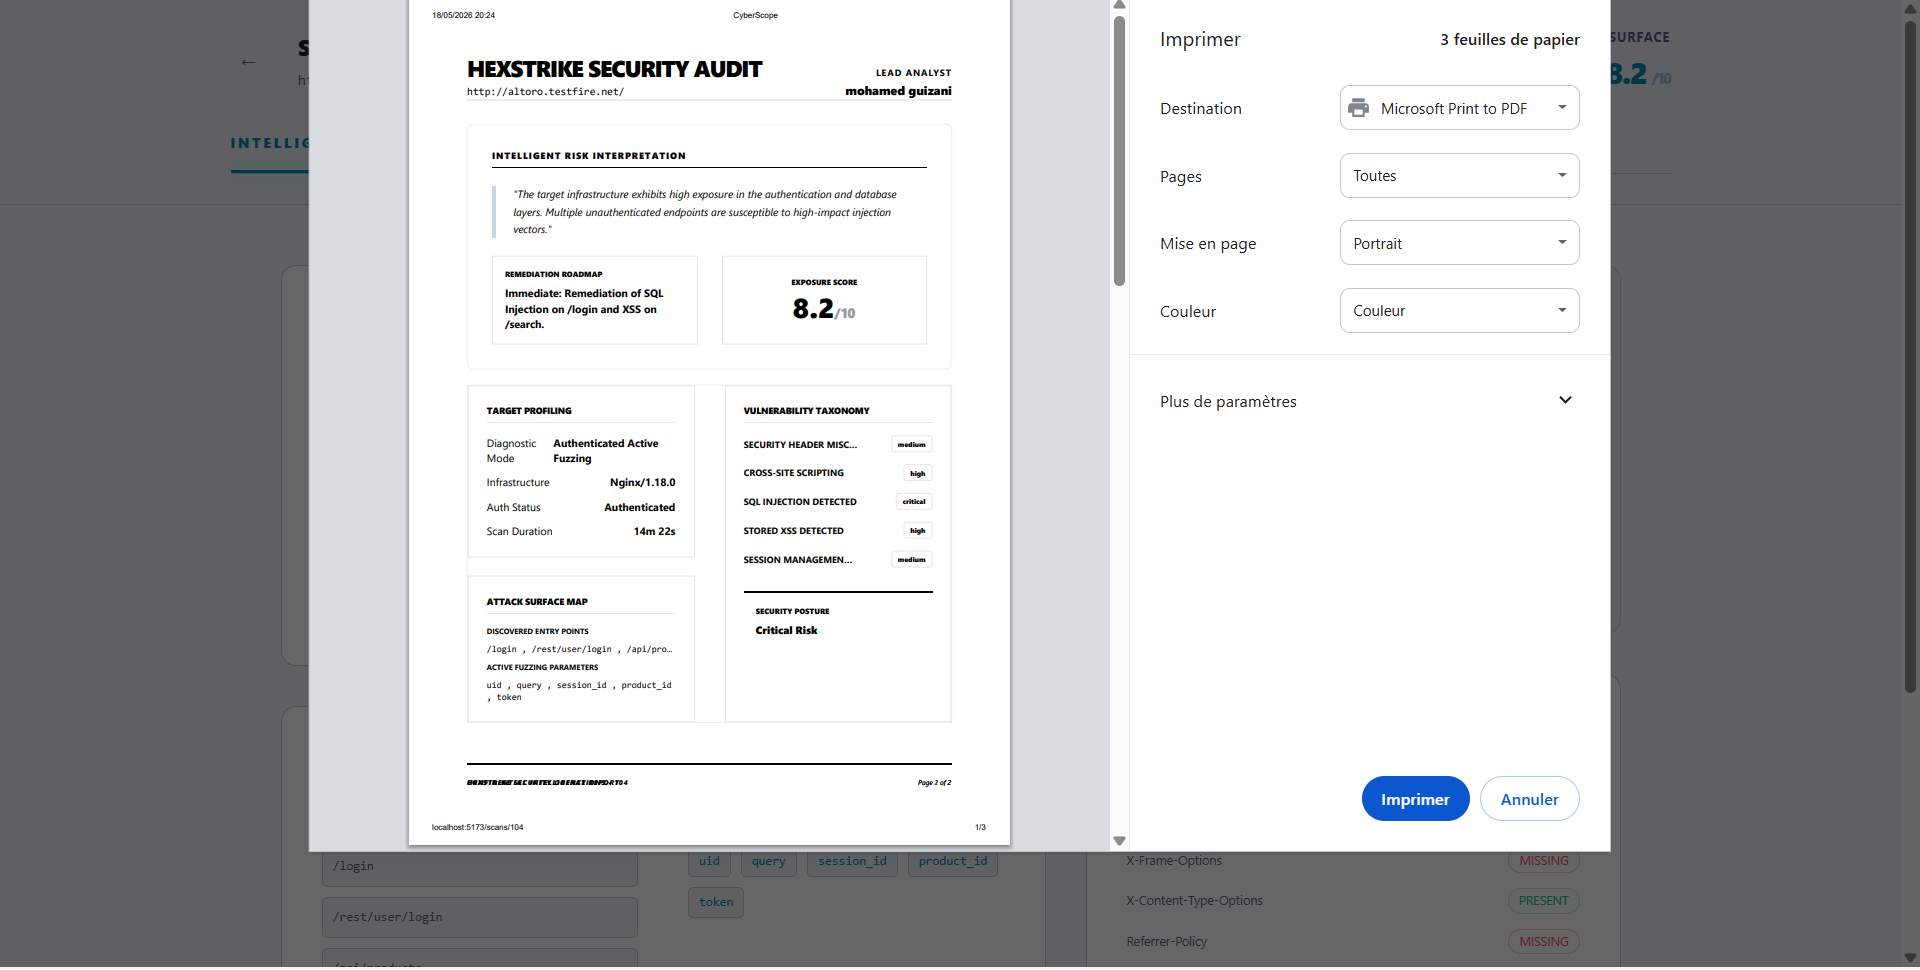
\includegraphics[width=0.85\textwidth]{uploads/images/export.png}}}% 
    \caption{export Scan Report page}
    \label{fig:export-scan-report}
\end{figure}

\begin{figure}[H]
    \centering
    \fbox{\parbox{0.85\textwidth}{\centering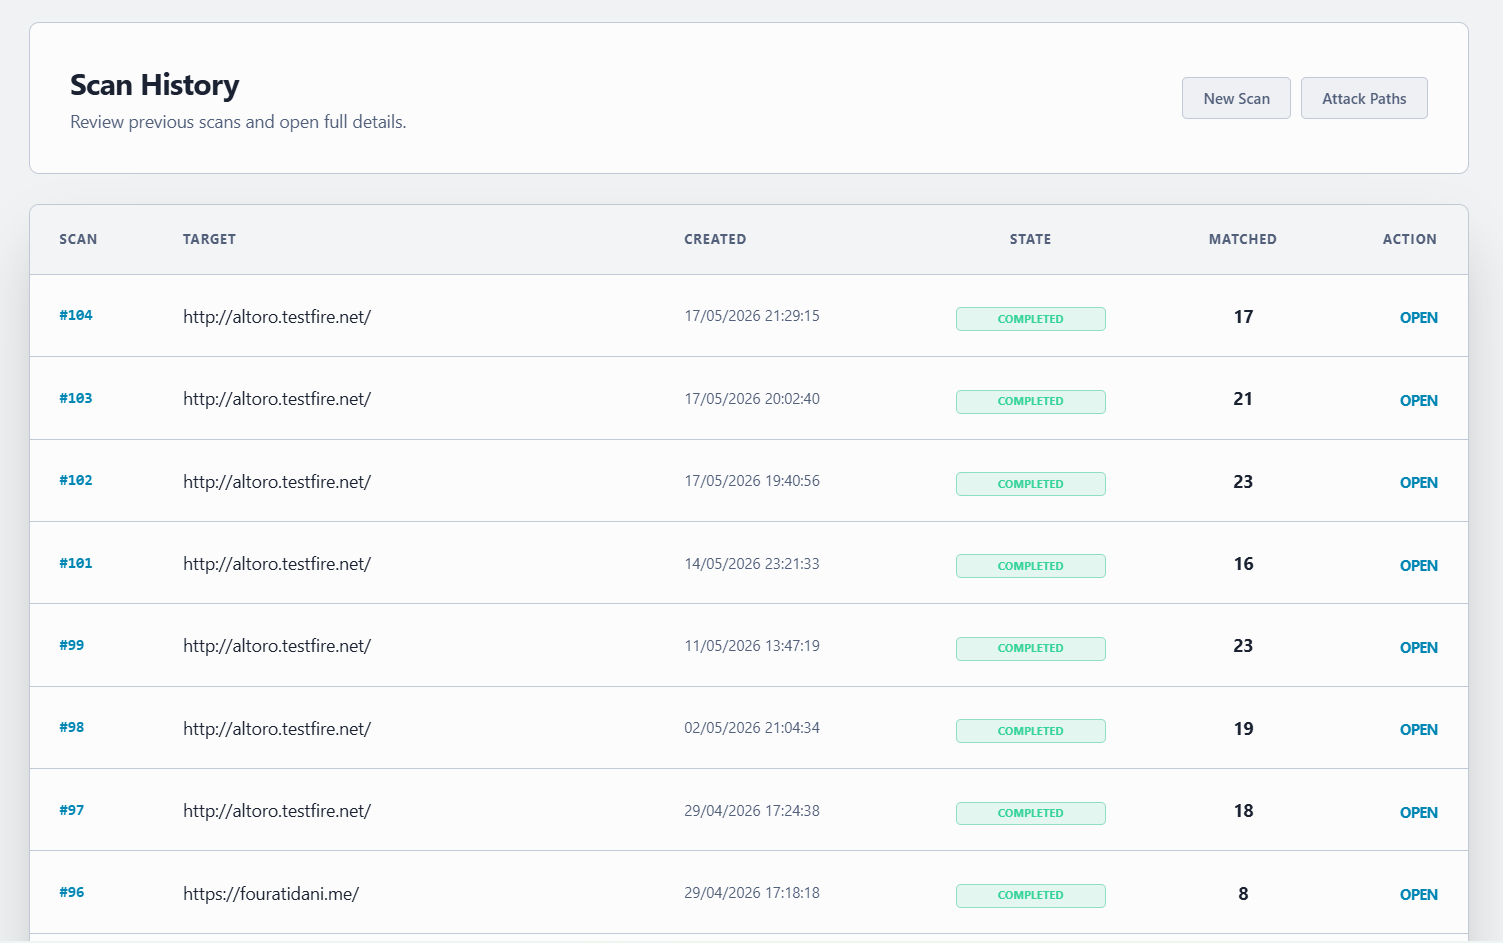
\includegraphics[width=0.85\textwidth]{uploads/images/scan history.png}}}% 
    \caption{Scan history page}
    \label{fig:scan-history4-page}
\end{figure}

\begin{figure}[H]
    \centering
    \fbox{\parbox{0.85\textwidth}{\centering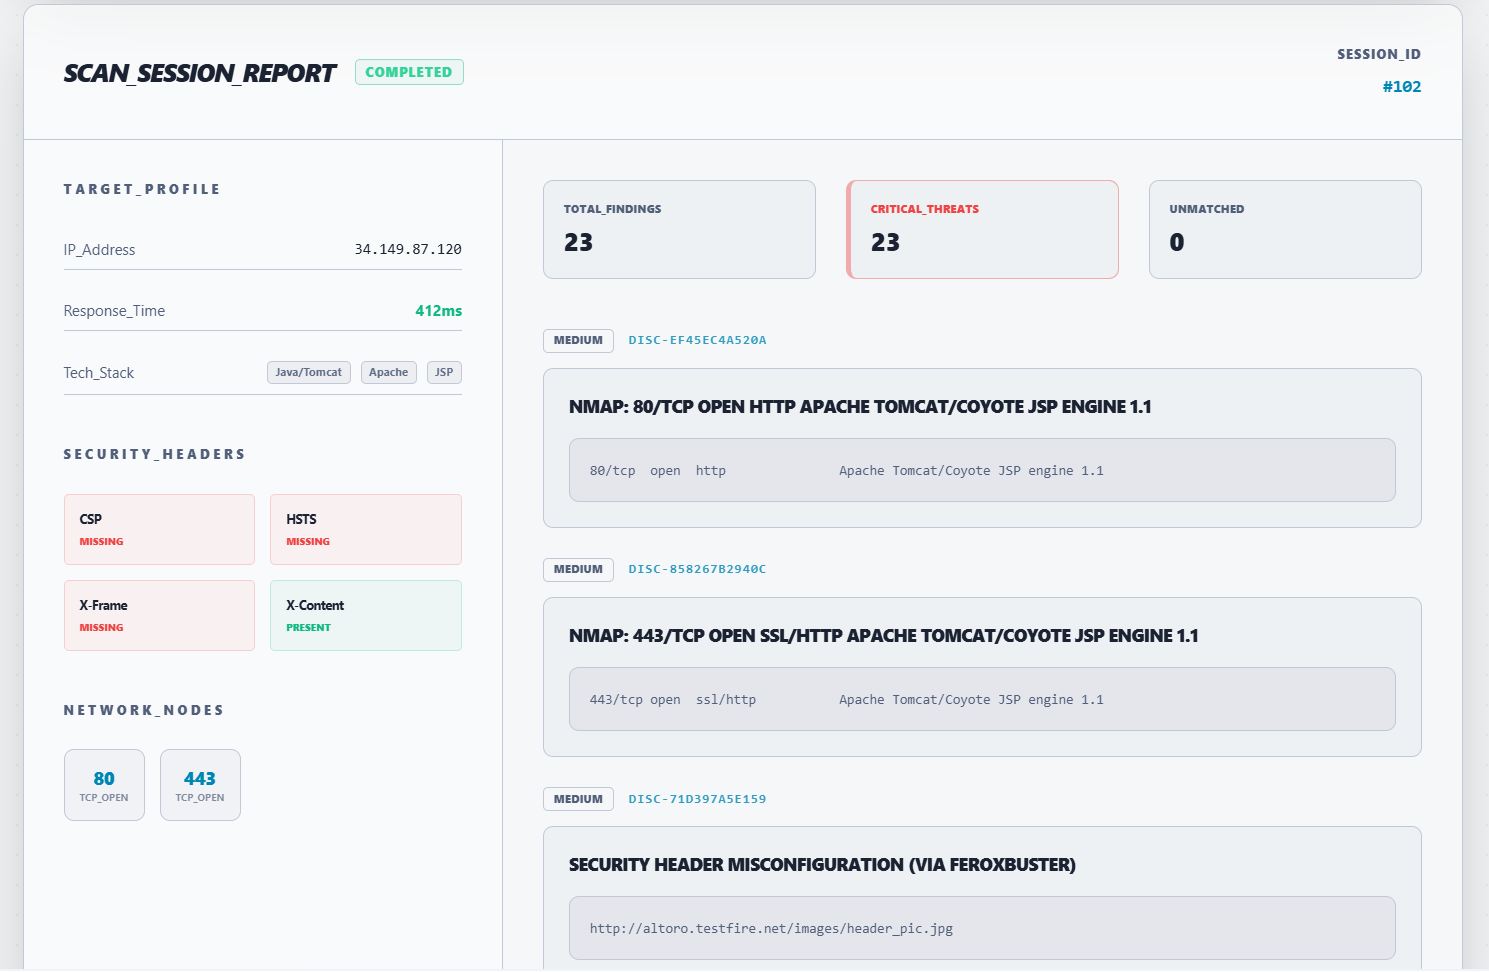
\includegraphics[width=0.85\textwidth]{uploads/images/scan result.png}}}% 
    \caption{Scan details page}
    \label{fig:scan-details4-page}
\end{figure}

\section{Conclusion}

This sprint builds the core scan processing pipeline and the infrastructure to normalize and match findings. With results persisted and accessible through the UI, future sprints can focus on reporting, enrichment, and advanced correlation features.
